\graphicspath{{chapters/02/}}
\chapter{Coverage}
\section{Local Coverage and Allelic Fraction}
Two key concepts needed when perfoming genomics analysis are the \textbf{local coverage} and \textbf{allelic fraction}.

	\paragraph*{Local coverage (cov)}
		The local coverage (cov) at position (base) $i$ is the number of reads that span $p_i$.
	\paragraph*{Allelic fraction (AF)}
		The allelic fraction (AF) at position $i$ is the proportion of reads that supports 			the reference base in $p_i$, and viceversa. 

The Lander-Waterman equation to compute NGS coverage is:
\begin{equation}
C = \frac{L * N}{G}
\end{equation}
Where G is the coverage, G is the haploid human genome length, L the read length and N the number of mapped reads.

\subsection{Mapping in NGS}
The number of mapped reads is always lower than expected. Errors, or major translocation will impair a good mapping of the reads. \\
There's a difference between physical and sequence coverage. Physical coverage is always higher, and it changes based on which protocol (PE or SE) is chosen for the assay.
To put it simply, when calculating the sequence coverage we only take into account the actual ends, while when calculating the physical coverage we also account for the consequence part of the PE protocol. In figure \ref{fig:seq_phys} a  shcematic representation of this problem is displayed.
\begin{figure}[htbp!]
    \centering
    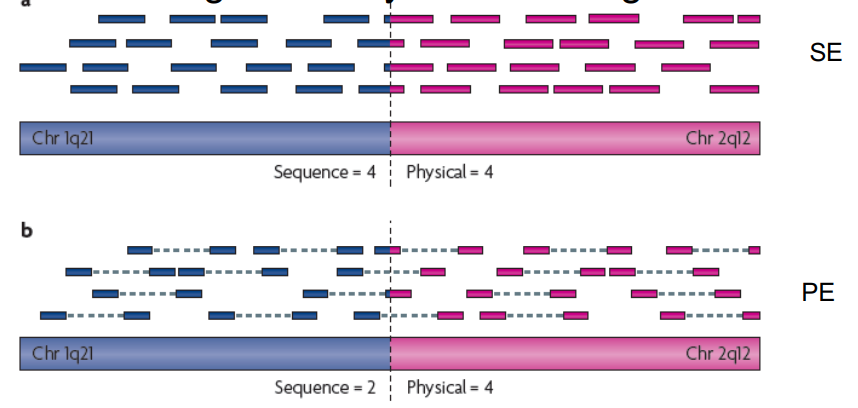
\includegraphics[width=0.5\textwidth]{seq_phys.png}
    \caption{Schematic difference between sequence (on the left) and physical coverage (on the right). From Meyerson et al., Nature Reviews Genetics 2010}
    \label{fig:seq_phys}
\end{figure}

Formal definitions of sequence and physical coverage are:

\paragraph*{Sequence coverage:}
	Sequence coverage is the amount of oversampling (how many times a base is sequenced); to detect nucleotide alterations with high sensitivity, the 3 billion bases of the human genome have typically been ‘covered’ with at least 30-fold (30X) on average, meaning 90 billion bases of sequence data per sample. 
	\paragraph*{Physical coverage:}
		the expected distance between the paired reads is used to uniquely place the reads on the genome; unexpected read pairs are used to detect structural anomalies.
		
		

\section{Tuning the intended coverage of a NGS assay}
In some experiments setups there's the need to carefully control the amount of intended coverage. \\
If we are looking for SNPs only, which by definition are present in all of the cells, we only need enough redundancy (local coverage) to detect them and distinguish the reference base and the alternative base (in case of an heterozygous SNP we will ideally find half of the reads supporting the reference and half supporting the alternatice). Indeed for SNPs we do not need more than 10-15 X coverage. 
\\
However, if the sample comes from a tumor or hematopoietic events, we need to look for subclonal events. Subclonal events are not harbored by all of the cells but only by a fraction of them. If we expect 1/4 of the cells harboring the mutation, we need to increase the coverage. \\
The same reasoning goes for any monozygous mutation and any low abundant events, and for  transcripts expressed at very low level (RNA-seq) and weak binding in ChIP-Seq. 

\subsection{Example on the importance of coverage}
Here are represented 10 genes relevant for cancer. Each bar represents the average local coverage at 30 bp.
\begin{figure}[htbp!]
    \centering
    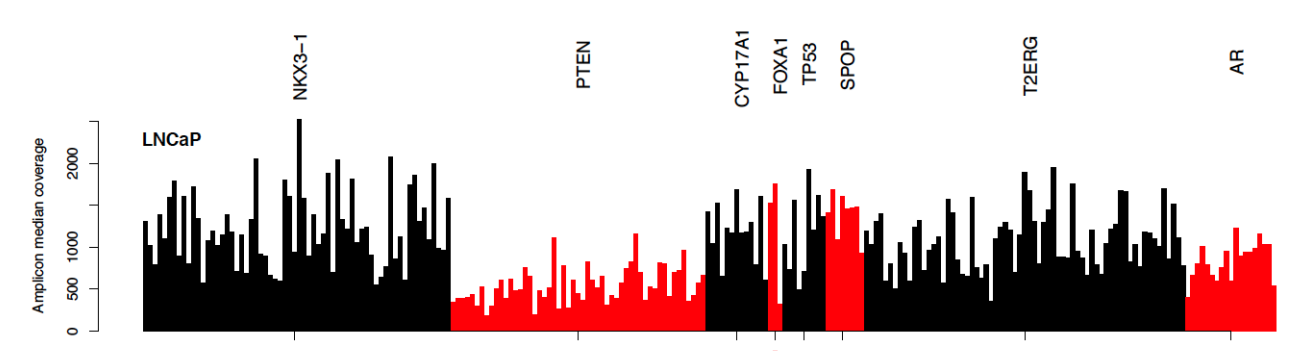
\includegraphics[width=0.5\textwidth]{local_coverage.png}
    \caption{Example of local coverage. On the x axis genomic location (on top e ery gene) and the bars is the number of amplicons. }
    \label{fig:local}
\end{figure}

In figure \ref{fig:local} a barplot can be observed, representing the local coverage (y axis) in the gene locations (x axis). The \textit{cov} is on average about 600x and it's "wavy", not evenly distributed (very typical). However, if one would do an average of the coverage for each gene, they would discover that one gene is abundantly underrepresented: PTEN.\\
What's happening on PTEN base on plot \ref{fig:local}? Probably, the most accurate guess is a deletion. But of which kind? For sure not a homozygous deletion, since we would not be able to see any signal in the plot. From this data however we cannot say whether this is a monoallelic or biallelic deletion. \\
Note that this (and the following \ref{fig:local2}) plot is the actual way sequencing data is shown, while the figure presented in \ref{SE_PE} was a schematic representation. 

\begin{figure}[htbp!]
    \centering
    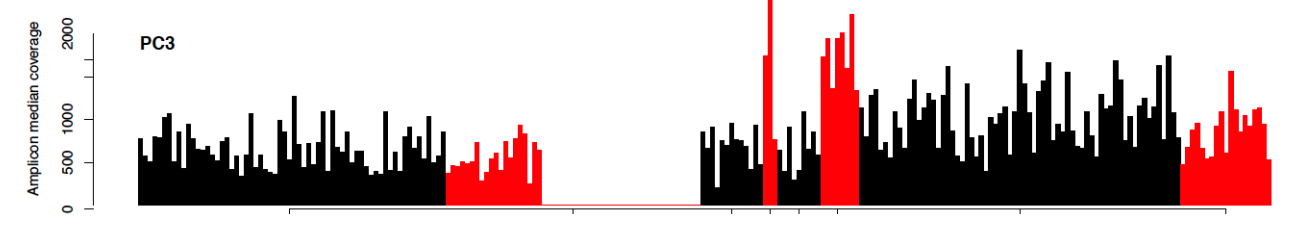
\includegraphics[width=0.5\textwidth]{local_coverage1.png}
    \caption{Example 2 of local coverage. The  cell line is different (PC3 instead of LNCaP). }
    \label{fig:local1}
\end{figure}

However, in the plot \ref{fig:local1}, from a different cell line, we can see a clear monoallelic deletion and a partial biallelic deletion of PTEN.\\

\begin{figure}[htbp!]
    \centering
    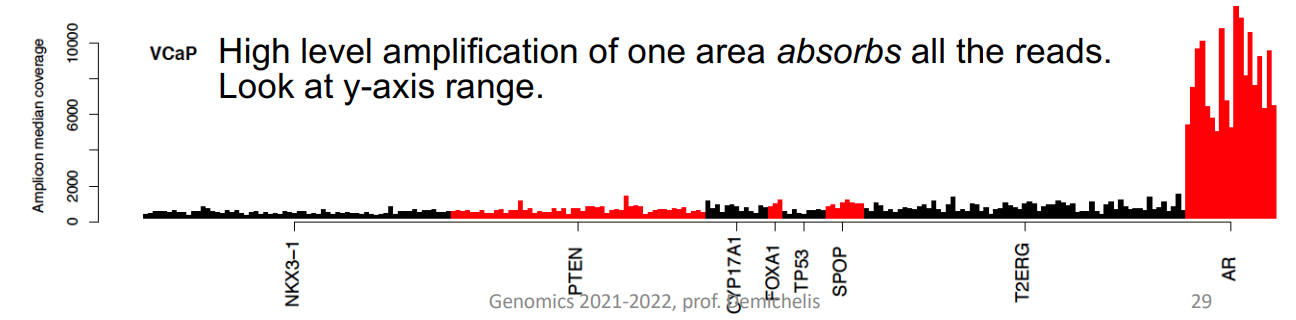
\includegraphics[width=0.5\textwidth]{local_coverage2.png}
    \caption{Example 3 of local coverage. The  cell line is different (VCaP). The massive amplification of the AR region is typicall in advanced prostate cancer.}
    \label{fig:local2}
\end{figure}

In figure \ref{fig:local2} we can see a massive amplification of the antigen receptor. Probably it was a mistake in the assay: amplification on the AR does not allow the analysis/discovery of other copy number variations because all of the reads will go to the AR site. \\
These were amplicon-based approaches. 
With NGS instead, It is easy to increase the experimental coverage (i.e. the sequence depth) at later point in time. 
Provided our original sample/library is still available, we can perform another run of sequencing and then combine the output from different runs. 
Note that this isn’t possible with array-based technologies.\\
However, there are some limiting factors of NGS DNA-seq experiments. 
Problems with repeated regions, but also not knowing the linearity of the genome. 
If the sequencing is done with longer reads we could tackle the problem by having longer molecules to work with, but there are more errors in the reads. 

\subsection{Databases}
Two very known databases for NGS analysis are:
\begin{itemize}
\item \textbf{Genome Reference Consortium}: assemble a reference genome reflecting the most common sequences in population at each position while tracking information on polymorphisms. 
\item \textbf{USCS Genome Browser}: select a reference genome and query all known features.
\end{itemize}

\section{Interpreting Pair Orientations}
We will now look at some aberrations' discoveries performed using IGV.\\
In IGV, each vertical bar corresponds to a read. 
If there is a colored sign, there is a polymorphism or difference with respect to a reference. 
The bowser also gives info about the quality of the read and bases (and others from the BAM file).\\
While using a paired-end protocol, we can study inversions, duplications and translocations. A useful legend to navigate the subsequent example is reported in the list below.
\begin{itemize}
\item \textbf{LR} ($\rightarrow \, \, \, \leftarrow$): Illumina (convention), the reads are left and right of the unsequenced part of the sequenced DNA fragment when aligned back to the reference genome;
\item \textbf{LL}, \textbf{RR}: implies inversion in sequenced DNA with respect to reference ;
\item \textbf{RL}: implies duplication or translocation with respect to reference;

\end{itemize}

\subsection{Inversion}
To detect major aberration, like inversions, we need reads that span the breakpoint (either long reads, or, better, PE reads). \\
What's happening exactly at the breakpoint in figure \ref{fig:inversion}? What's the coverage when looking at the data?  When we map them on the reference, we see that the direction is LL and RR, meaning that there is an inversion.
%The sequence that we have in the molecule does not exist there and therefore that sequence doe not exist in two copies in the molecule. 
We can also spot a drop in the local coverage.  
In the target molecule, either it does not exist or exist only in one allele and not the other one. \\
When interpreting structural variance, we need not to care only about end-orientation, but also coverage at the exact break point, which is due to the fact that the inverted breakpoint sequence does not exist in the reference genome.


\begin{figure}[htbp!]
    \centering
    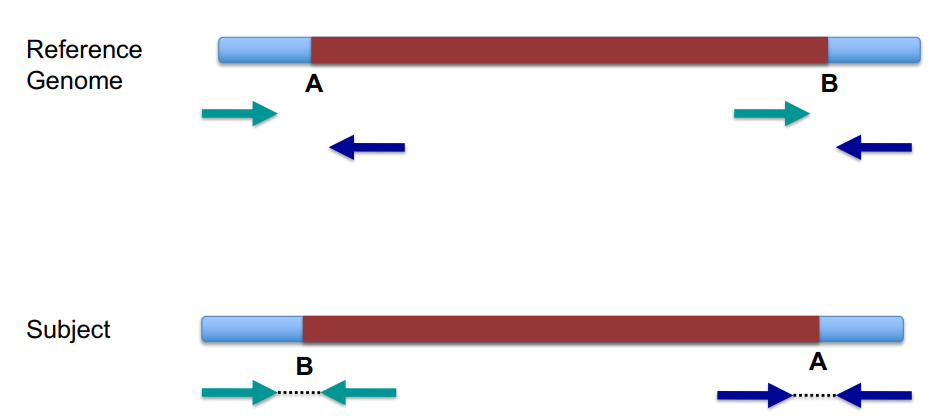
\includegraphics[width=0.5\textwidth]{inversion.png}
    \caption{Inversion disocvering exploiting PE reads.}
    \label{fig:inversion}
\end{figure}


\subsection{Tandem duplication}
Notice how in the tandem duplication (figure \ref{fig:tandem}) all the reads that do not cover the junction point align perfectly to the reference.
The coverage will be 3/2 of the expected value, proportional to the extra copy. B junction and A junction will not have modifications. If we had a read mapping BA, we would observe a partial alignment at B on the reference.
We observe no drop of coverage because the sequences also exist in the reference. \\

\begin{figure}[htbp!]
    \centering
    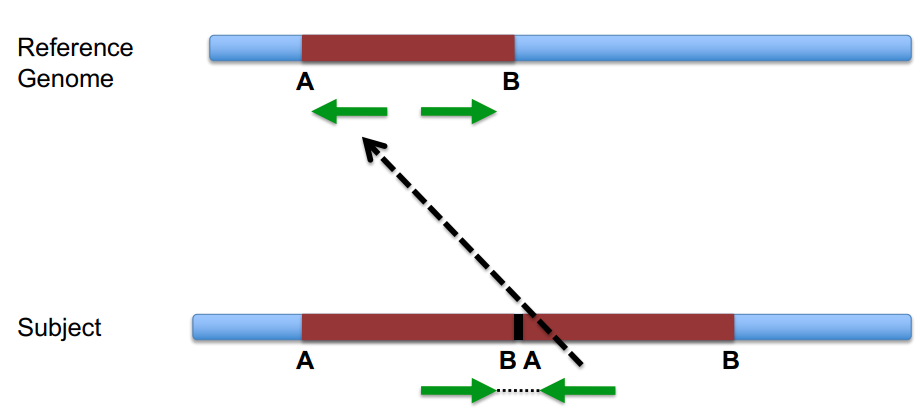
\includegraphics[width=0.5\textwidth]{tandem.png}
    \caption{Tandem duplication discovering exploiting PE reads.}
    \label{fig:tandem}
\end{figure}

\subsection{Inverted duplication}
For the inverted duplication, in figure \ref{fig:inverted, we expect double coverage in the duplicated site in the reference genome. \\
Both A and B on the first segment on the subject are LR oriented, and the same occurs in the reference genome. 
When we add the second fragment the same holds, but direction will be LL and RR and the insert size will be significantly longer. In particular, we can notice that we have an overlapping of left and right reads on the reference. Furthermore, the coverage depth will highly increase due to the presence of multiple reads on the reference genome.

\begin{figure}[htbp!]
    \centering
    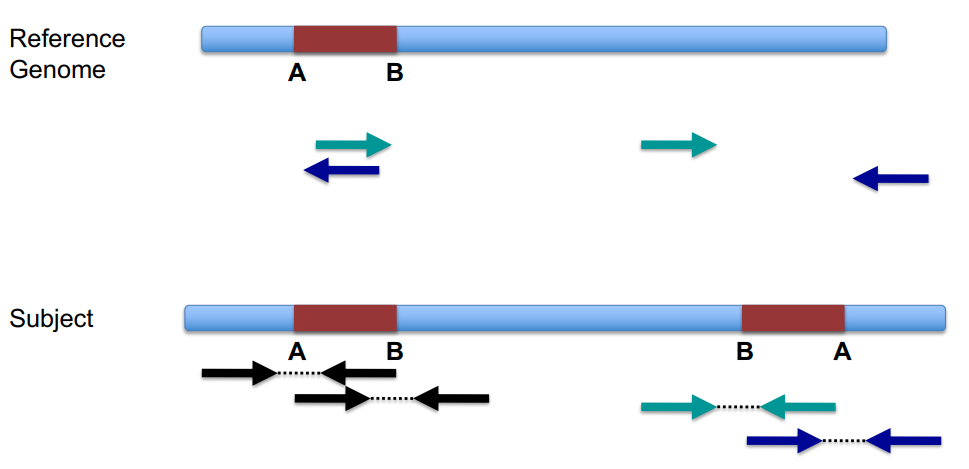
\includegraphics[width=0.5\textwidth]{inverted.png}
    \caption{Inverted duplication discovering exploiting PE reads.}
    \label{fig:inverted}
\end{figure}

What if we have a deletion? How can you guess the size of it? We can look at the coverage or observed distance between the reads, which gives clean indication of the size of the deletion. For tiny deletions, smaller than the length of the read, we use the sequence within the reads and in this way discovering indels.  

\section{Summary}
Summarizing, the elements to consider are:
 \begin{itemize}
 \item Pair ends relative orientation;
 \item Insert size length; 
\item Coverage within the aberrant region; 
\item Coverage outside of the aberrant region (flanking genomic segments); 
\item Coverage at the breakpoints. 
 \end{itemize}





 
















